% IDEAS
% - Comparar C vs ASM:
%   - Imágenes: deberian ser identicas salvo randomness
%   - Velocidad: ASM debería ser más rápido
% - Comparar con Mongi (C vs C y ASM vs ASM):
%   - Imágenes para el mismo setup, como son las imagenes generadas (visualmente)
%   - Velocidad: usar los mismos casos de prueba del informe de Mongi para
%     comparar los tiempos de ejecucion en esos casos
% - Comparar con implementacion original:
%   - Imágenes para el mismo setup (deberian ser identicas, salvo randomness)
%   - Velocidad: debería ser mas rápido

\section{Experimentación}

En esta sección pondremos a prueba a ambos Ray Tracer, y los compararemos entre
sí en diferentes escenarios para ver si efectivamente el uso de instrucciones
SIMD mejora el rendimiento de los mismos.

Todos los experimentos se corrieron en una notebook HP 14-dk1003dx, que cuenta
con una CPU AMD Athlon Silver 3050U de 2.3GHz, 1MB de cache L2, y 16GB de RAM.
El sistema corre Arch Linux, y utiliza la versión 6.7.5 de linux. Los binarios
en C y en ASM se compilaron con GCC v13.2.1 y con NASM v2.16.01 respectivamente.

\subsection{Diferencia entre implementaciones}

En este primer experimento, generaremos imágenes para escenas similares usando
las distintas implementaciones que tenemos a disposición: el ray tracer de
Mongi, el original en C++, y el desarrollado en ASM (el que está hecho en C
genera exactamente las mismas imágenes). La motivación es tener una idea general
de como se diferencian los ray tracers, y además una medida del tiempo que tarda
cada uno en generar la imagen de la escena.

Por la diferencia en cómo esta implementado cada uno, esperamos que el de Mongi
sea el más rápido, y el original en C++ el más lento. La implementación de Mongi
usa una simplificación para el cálculo del color, en vez de ``rebotar'' el rayo
por la escena hasta llegar a una fuente de luz y combinar los aportes de todas
las superficies, en la primer intersección se calcula el aporte de cada fuente
de luz con la superficie.

\begin{figure}
    \centering
    \begin{subfigure}[b]{0.45\textwidth}
        \centering
        \includegraphics[width=\textwidth]{../images/impl_diffs/mongi-sphere.png}
        \caption{Implementación de Mongi}
        \label{fig:yellow-sphere-mongi}
    \end{subfigure}
    \hfill
    \begin{subfigure}[b]{0.45\textwidth}
        \centering
        \includegraphics[width=\textwidth]{../images/impl_diffs/asm-sphere.png}
        \caption{Implementación en ASM}
        \label{fig:yellow-sphere-asm}
    \end{subfigure}
    \hfill
    \begin{subfigure}[b]{0.45\textwidth}
        \centering
        \includegraphics[width=\textwidth]{../images/impl_diffs/cpp-sphere.png}
        \caption{Implementación original en C++}
        \label{fig:yellow-sphere-cpp}
    \end{subfigure}

    \caption{Escena de una esfera amarilla sobre una superficie gris}
    \label{fig:yellow-sphere}
\end{figure}

En la figura \ref{fig:yellow-sphere} podemos ver las imágenes generadas. La de
Mongi (\ref{fig:yellow-sphere-mongi}) es claramente distinta por lo que ya
explicamos anteriormente, se puede ver como tanto el ángulo de incidencia, como
la distancia de la intersección a la luz afectan a su aporte en la imagen,
haciendo que algunas partes se vean más oscuras. Por otro lado, las
implementaciones en ASM (\ref{fig:yellow-sphere-asm}) y en CPP
(\ref{fig:yellow-sphere-cpp}) generan imágenes muy parecidas, y más iluminadas
que en la primer imagen.

La diferencia de color que se puede apreciar entre éstas últimas se debe a cómo
están iluminadas. En ASM usamos un plano a cierta altura para que simule una luz
solar, mientras que en C++ los rayos que no colisionan con ningún objeto toman
un color predeterminado que depende de su dirección.

Los tiempos de ejecución los obtenemos realizando 10 mediciones y tomando el
promedio. Usamos el comando `time` que se puede encontrar en la mayoría de
distribuciones de Linux. El tiempo CPU es el tiempo que el programa estuvo
ejecutando, mientras que el Real es el tiempo real que transcurrió desde que
empezó la ejecución hasta que termino (puede incluir esperas de IO,
manejo de interrupciones, etc.)

\begin{itemize}
    \item Mongi:
        \begin{itemize}
            \item CPU: 328.4 ms
            \item Real: 365.3 ms
        \end{itemize}
    \item ASM:
        \begin{itemize}
            \item CPU: 4326.8 ms
            \item Real: 4361.8 ms
        \end{itemize}
    \item C++:
        \begin{itemize}
            \item CPU: 14986.5 ms
            \item Real: 15052.3 ms
        \end{itemize}
\end{itemize}

Como podemos ver, los resultados concuerdan con nuestras suposiciones iniciales.
Mongi es casi 13 veces más rápido que ASM, y ASM 3.5 veces más rápido que C++.

Si bien la diferencia es sustancial, es importante recordar que los ray tracer
en ASM y C++ pueden parametrizar opciones como \texttt{spp} y
\texttt{max\_depth}, mientras que el de Mongi los tiene fijados en 1 por
definición. Si corremos nuevamente ASM pero con un \texttt{spp=1} y
\texttt{depth=5}, podemos obtener un tiempo de ejecución de 350 ms sacrificando
la calidad de la imagen.


\subsection{Tiempos de ejecución con escena preparada para distintas
resoluciones}

Inspirado en el experimento realizado por Mongi en su trabajo, compararemos los
tiempos de ejecución de las implementaciones en C y ASM para una misma escena,
pero variando la resolución de la imagen de salida. Se espera que ASM sea
ampliamente superior a C en este aspecto.

\begin{figure}
    \centering
    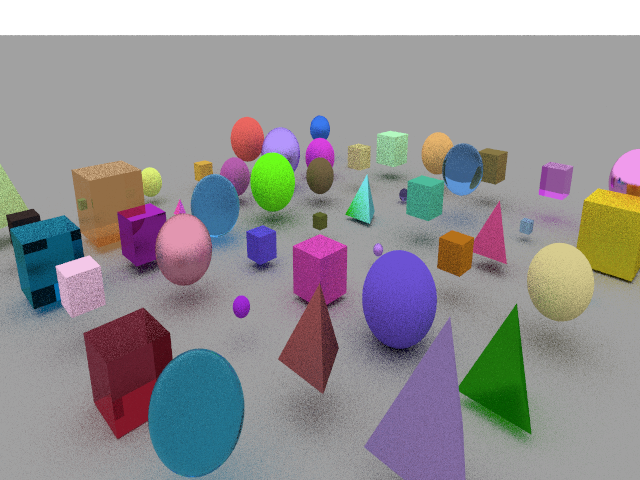
\includegraphics[width=\textwidth]{./imgs/exp2-scene.png}
    \caption{Escena a utilizarse para la medición}
    \label{fig:exp2-scene}
\end{figure}

Usaremos la escena que se muestra en la figura \ref{fig:exp2-scene} para
realizar las mediciones usando las opciones \texttt{-m 1 -n 3} del programa, que
le indica realizar 3 mediciones de tipo 1 (cantidad de ciclos de clock), y
obtener el promedio.

\begin{figure}
    \centering
    \begin{subfigure}[b]{0.45\textwidth}
        \centering
        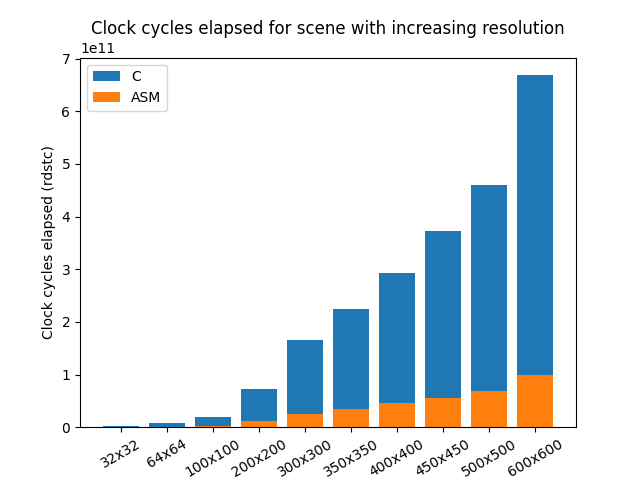
\includegraphics[width=\textwidth]{./imgs/exp2-res-bar.png}
        \caption{Ciclos de clock por resolución}
        \label{fig:exp2-res-bar}
    \end{subfigure}
    \hfill
    \begin{subfigure}[b]{0.45\textwidth}
        \centering
        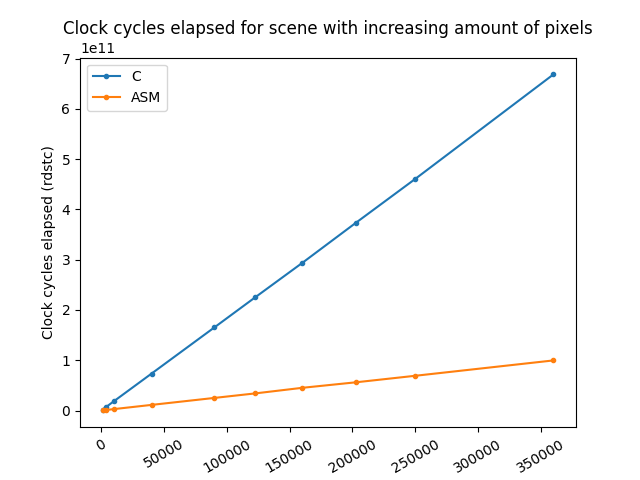
\includegraphics[width=\textwidth]{./imgs/exp2-res-line.png}
        \caption{Ciclos de clock por cantidad de pixeles}
        \label{fig:exp2-res-line}
    \end{subfigure}
    \caption{Resultado del experimento en 2 formatos}
    \label{fig:exp2-res}
\end{figure}

En la figura \ref{fig:exp2-res} podemos ver el resultado en 2 formatos. En
\ref{fig:exp2-res-bar} vemos como en cada resolución, ASM requiere de muchos
menos ciclos para generar la misma imagen que en C. Por otro lado, en
\ref{fig:exp2-res-line} se puede ver como estas magnitudes crecen de forma
lineal respecto a la cantidad de pixeles de cada imagen, lo cual tiene sentido.

\subsection{Tiempos de ejecución por tipo de objeto para distintas cantidades}

% generar escenas por cada tipo de objeto que contengan solo ese tipo, y variar
% la cantidad de objetos de la escena, y ver la variación de tiempo por cada
% uno.

\subsection{Tiempos de ejecución por tipo de material para distintas cantidades}

% idem pero por cada tipo de material. Usar esferas ya que son más simples y asi
% las escenas tienen cierta uniformidad.

\subsection{Variación de depth vs. spp para una escena preparada}

% Ver como varía la imagen para distintos depth y spp, y elegir una
% configuración óptima que no sacrifique mucha calidad de imagen
